\documentclass{sigchi}

% Remove Fake Conference information
\renewcommand\footnotetextcopyrightpermission[1]{} % removes footnote with conference information in
\pagestyle{plain} % removes running headers
\acmDOI{}

% Load basic packages
\usepackage{balance}       % to better equalize the last page
\usepackage{graphics}      % for EPS, load graphicx instead 
\usepackage[T1]{fontenc}   % for umlauts and other diaeresis
\usepackage{txfonts}
\usepackage{mathptmx}
\usepackage[pdflang={en-US},pdftex]{hyperref}
\usepackage{color}
\usepackage{booktabs}
\usepackage{textcomp}

% Some optional stuff you might like/need.
\usepackage{microtype}        % Improved Tracking and Kerning
% \usepackage[all]{hypcap}    % Fixes bug in hyperref caption linking
\usepackage{ccicons}          % Cite your images correctly!
% \usepackage[utf8]{inputenc} % for a UTF8 editor only

% Paper metadata (use plain text, for PDF inclusion and later
% re-using, if desired).  Use \emtpyauthor when submitting for review
% so you remain anonymous.
\def\plaintitle{Software Dependability Analysis - Apache Commons Validator Library}
\def\plainkeywords{Apache Commons Validator; SonarCloud; Code Coverage; PiTest, Mutation Testing; Java Microbenchmark Harness, JMH; Test Coverage; EvoSuite; Automated Test Case Generation; FindSecBugs, Security Analysis; OWASP, Vulnerability Detection; Dependability.}
\def\plainauthor{Katia Melanie Perchet}

\renewcommand{\shortauthors}{Katia M. Perchet}

% To make various LaTeX processors do the right thing with page size.
\def\pprw{8.5in}
\def\pprh{11in}
\special{papersize=\pprw,\pprh}
\setlength{\paperwidth}{\pprw}
\setlength{\paperheight}{\pprh}
\setlength{\pdfpagewidth}{\pprw}
\setlength{\pdfpageheight}{\pprh}

% Make sure hyperref comes last of your loaded packages, to give it a
% fighting chance of not being over-written, since its job is to
% redefine many LaTeX commands.
\definecolor{linkColor}{RGB}{6,125,233}
\hypersetup{%
  pdftitle={\plaintitle},
% Use \plainauthor for final version.
 pdfauthor={\plainauthor},
  pdfkeywords={\plainkeywords},
  %pdfdisplaydoctitle=true, % For Accessibility
  bookmarksnumbered,
  pdfstartview={FitH},
  colorlinks,
  citecolor=black,
  filecolor=black,
  linkcolor=black,
  urlcolor=linkColor,
  breaklinks=true,
  hypertexnames=false
}

\makeatletter
\def\@copyrightspace{\relax}
\makeatother
% End of preamble. Here it comes the document.
\begin{document}

\title{Software Dependability Analysis - Apache Commons Validator Library}

\author{
  \alignauthor{Katia Melanie Perchet\\
    \affaddr{Università degli Studi di Salerno}\\
    \affaddr{Fisciano, Salerno, Italy}\\
    \email{k.perchet@studenti.unisa.it}}\\
}

\maketitle


\begin{abstract}
  This paper presents an analysis of the software dependability of the Apache Commons Validator Library leveraging a multi-faceted approach, employing various tools and techniques such as SonarCloud, code coverage analysis with JaCoCo and CodeCov, PiTest mutation testing, Java Microbenchmark Harness (JMH), EvoSuite, FindSecBugs, and OWASP. The investigation delves into SonarCloud for static code analysis and resolution of issues, Code Coverage for assessing the extent of test coverage, PiTest for mutation testing to identify code weaknesses, JMH for performance characteristics, EvoSuite for automated test case generation, FindSecBugs for security analysis, and OWASP for vulnerability detection. 
  Through this combined methodology, it is aim to provide a comprehensive evaluation of the library's dependability, addressing aspects of code quality, test coverage, security, and performance. This analysis contributes to enhancing the reliability and robustness of the Apache Commons Validator library, offering valuable insights to pursuit a reliable and robust software system.
\end{abstract}
% Author Keywords
\keywords{\plainkeywords}
\section{1. Introduction}

In an era where software applications form the backbone of various industries, the demand for robust, dependable code has never been more critical. Within this context, the Apache Commons Validator library stands as a cornerstone for Java developers, providing essential tools for data validation. Recognizing the importance of software dependability, this paper embarks on an exhaustive exploration, employing a cutting-edge tools and methodologies to inspect the inner workings of this foundational library.

The primary objective is to conduct a thorough analysis that spans multiple dimensions of software dependability. To achieve this, diverse set of tools will be used, each designed to unveil distinct aspects of the library's performance. SonarCloud, a dynamic static code analysis tool, offers insights into code quality and architecture. Code coverage analysis provides a lens into the efficacy of the test suite, ensuring comprehensive coverage through JaCoCo and CodeCov. PiTest, a mutation testing tool, allows to identify potential code weaknesses by dynamically altering the production code and observing test outcomes.

Java Microbenchmark Harness (JMH) provides information about the library's performance characteristics, addressing vital questions surrounding efficiency and speed. EvoSuite, an automated test case generation tool, aids in fortifying the library's resilience by systematically generating test cases. FindSecBugs, dedicated to security analysis, ensures that potential vulnerabilities are unearthed and addressed.

In sequence with these tools, the Open Web Application Security Project (OWASP) acts as a vigilant guardian, inspecting the library for potential security pitfalls. This combined approach forms a robust methodology, providing a perspective on the Apache Commons Validator library's dependability. It aims not only to identify and rectify potential weaknesses but also to contribute valuable insights.

In summary, this paper delves into diverse aspects of software dependability, extending beyond conventional boundaries.  It encompasses project analysis, analytics, testing tools, and vulnerability assessments, emphasizing the significance of reliability, security, and robustness in software systems. The focus remains on upholding the standards of dependability within the continually evolving realm of Java development. 

\subsection{1.1 Apache Commons Validator}
Apache Commons Validator \cite{apache-commons-validator} is an open-source Java library which can be found within the Apache Commons project. The library provides the ability to verify the integrity of incoming data, offering a versatile set of building blocks for both client-side and server-side data validation. 

It was designed for standalone use or seamless integration with frameworks, providing a robust solution for effectively streamline the often-repetitive process of data validation and caters to locale-specific rule application, ensuring a consistent approach across diverse sets of validation requirements.

The adoption of Apache Commons Validator brings a transformative approach to data validation, offering developers the means to overcome the complexities associated with diverse validation rules. By promoting efficiency in development processes, this solution contributes to maintaining high data integrity and providing an optimal user experience. 

In conclusion, as the data-driven applications continues to evolve, the role of Apache Commons Validator becomes increasingly vital in establishing robust, locale-aware validation practices.


\section{2. SonarCloud}
Upon thorough analysis of the commons-validator project using SonarCloud \cite{sonarcloud}, the generated report revealed an extensible list of issues identified within the project.

\subsection{2.1 SonarCloud Report}
As indicated in the SonarCloud report, the identified issues have been systematically categorized into four distinct sections: reliability, maintainability, security, and security review. 

Each of these sections is further classified according to Software Quality, further subdividing them into security, reliability, and maintainability concerns. Additionally, issues may be classified based on Clean Code Attributes categories, including consistency, intentionality, adaptability, and responsibility.

The project had a "failed" Quality Gate due to five bugs risking the reliability, six hundred and forty four code smells affecting its maintainability and five security hotspots in the security review section. 

\begin{figure}[h!]
\centering
  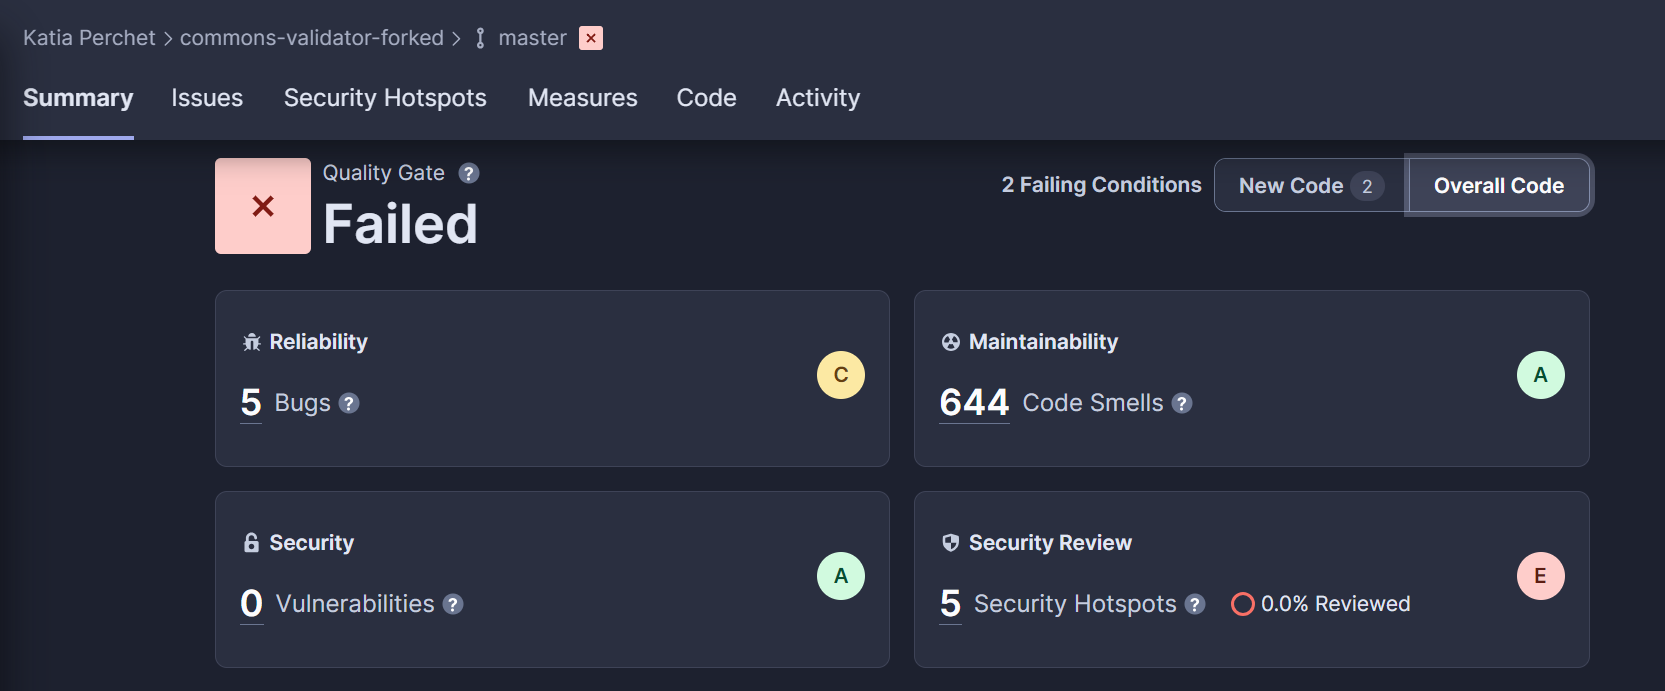
\includegraphics[width=1\columnwidth]{sonarcloudFail.png}
  \caption{Issues encountered.}~\label{fig:figure1}
\end{figure}

\subsubsection{\textbf{Reliability}}

\begin{itemize}
    \item \textbf{Medium - 3 issues.} There are only three issues related to the large regular expressions employed for the data validation, necessitated to enforce specified constraints, but might be leading to stack overflow.
    \item \textbf{Low - 2 issues.} Two issues are identified concerning the regular expressions utilized for data validation, specifically pertaining to the lack of coverage for empty strings moderation.  
\end{itemize}

\subsubsection{\textbf{Maintainability}}

\begin{itemize}
    \item \textbf{High - 36 issues.} Issues related to the implementation of "Clonable" Interface are observed, leading to concerns regarding the "clone" method due to instances of classes being instantiated without invoking their constructors, potentially resulting in unenforced preconditions. Furthermore, there are concerns regarding the Serializable class type, where certain fields lack the declaration as serializable or transient, introducing the possibility of application crashes and creates a vulnerability exploitable by attackers. 
    The report additionally showed the presence of empty methods lacking information or utility, evidencing bad practices. Another category of issues encountered is a large Cognitive Complexity in several methods, making the code hard to read, understand, test, and modify. 
    Moreover, there are identified issues concerning the absence of any assertions within specific test cases.
    \item \textbf{Medium - 150 issues.} Most of the issues identified in this category are associated to the extensive regular expressions found in the code. These expression, utilized for data validation, open the possibility of stack overflow for large inputs and a high code complexity. Furthermore, the reports draws the attention to several concerns: the presence of many nested try-catch blocks, making unclear the functionality of the code, inappropriate visibility of constructors, character duplication, incorrect assertion types, misplacement of method arguments and lack of code re-usability. 
    \item \textbf{Low - 458 issues.} Within this category, recommendations were provided to enhance the clarity and comprehensibility of the code. These include the identification of deprecated and commented out code for removal. The identification and mitigation of "Brain Method" occurrences to reduce code complexity and the detection of "Singleton" pattern to define if its needed. Further recommendations advise the removal of unnecessary boolean literals and adjustment of "public" modifier in test cases where its visibility is implicit. 
\end{itemize}

\subsubsection{\textbf{Security Hotspots}}
\begin{itemize}
    \item \textbf{Medium - 5 issues.} Suggestions to oversee the employed regular expression in this context, to ensure that Denial of Service is not the vulnerability to polynomial runtime issues attributed to the backtracking that regular expression's engines use. 
\end{itemize}



\subsection{2.2 Issues Fixed}
The fixing started based on the category errors, starting with the bugs that were affecting the reliability of the project, followed by the code smells that affected the maintainability of the code. It was attempted to address the majority of them, of which four of the bugs were fixed and five hundred and fifty one code smells, improving the clarity and comprehensibility of the code, leading to a "Passed" Quality Gate from SonarCloud's final report. 
\begin{figure}[h!]
    \centering
    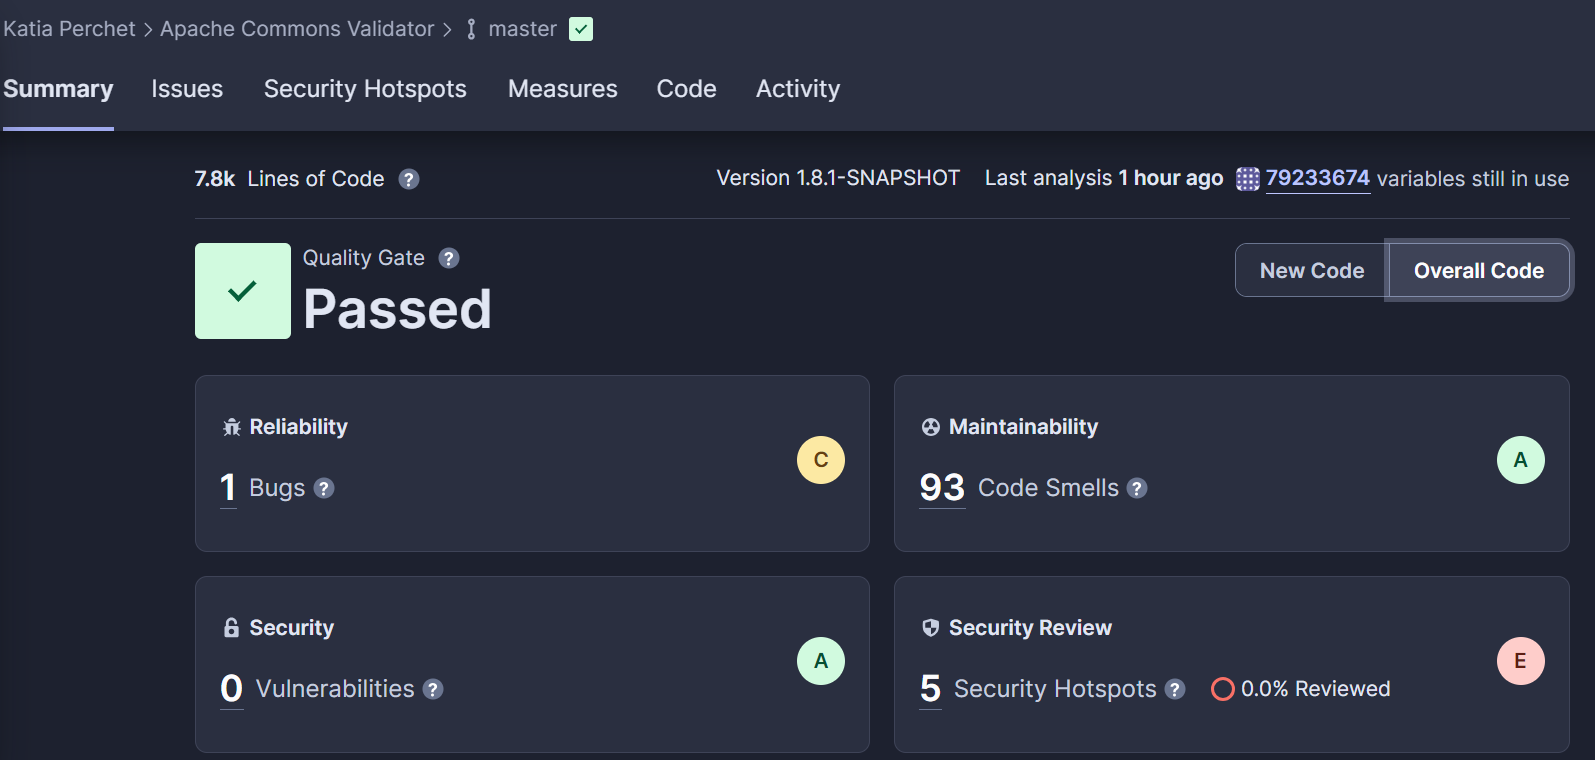
\includegraphics[width=1\columnwidth]{finalSonarCloud.png}
    \caption{Issues fixed.}
    \label{fig:enter-label}
\end{figure}

In addressing the identified bugs, four resolutions have been implemented. Specifically, two of these resolutions involved the truncation of regular expressions to avoid overflow when handling large inputs. The remaining two resolutions involved refactoring the regular expressions to prevent the acceptance of empty strings. 

On the other hand, to resolve the code smells, different approaches had been used:
\begin{itemize}
    \item 60\% of them were approached by removing the "public" modifier in test cases because the visibility is implied.
    \item 11\% of them were resolved by swapping the parameters in those methods where the arguments were inverted. 
    \item 4\% of them were approached by selecting the correct assertion type to match in the test cases and adding assertions when needed.
    \item 3\% of them were fixed by deleting commented code and to-do description tasks. 
    \item 2\% of them were addressed by simplifying the if-statements and returning expressions in methods. 
    \item 1\% of them were fixed by removing the "deprecated" tag from those variables that are still in use.
\end{itemize}


\section{3. Code Coverage}

The heading of this section is devoted to measuring the coverage of unit or integration tests, and assessing the reliability of the Apache Commons Validate project through the utilization of testing tools. The analysis begins with the examination of the code coverage using JaCoCo and CodeCov, clarifying their significance and influence. 

\subsection{3.1 JaCoCo}

JaCoCo (Java Code Coverage) \cite{jacoco} plays a substantial role when it comes to evaluating code coverage in Java applications. It offers valuable insights into the code execution during testing by generating a comprehensive reports that pinpoint to specific sections of the code exercised by the tests, providing a more specific area to focus on.
The report generated through JaCoCo's execution for all project packages revealed an Instruction Coverage baseline of 86\%. This signifies that only 2859 out of 211182 lines of code were not executed. 
Additionally, the report indicated a Branches Coverage of 74\%, revealing that 442 out of 1762 if or switch statements were missed. Further specific metrics include 482 out of 1681 missed cyclomatic complexities, 665 out of 3069 missed lines, 144 out of 787 missed methods, and 2 out of 76 missed classes.
\begin{figure}[h!]
    \centering
    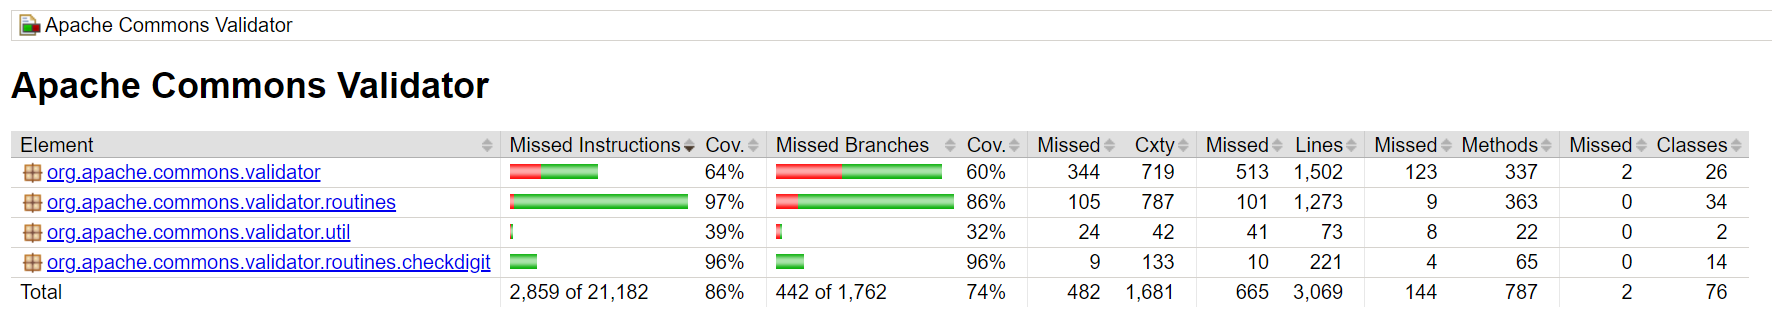
\includegraphics[width=1\columnwidth]{jacocoReport.png}
    \caption{JaCoCo generated report.}
    \label{fig:enter-label}
\end{figure}
The JaCoCo-generated report unveiled varying percentages for each package within the project.
\subsubsection{\textbf{Instruction Coverage}}
The Instruction Coverage section supplied details regarding the executed code, pointing out that the "routines" package demonstrated the highest code execution with the least amount of code missed.
\begin{itemize}
    \item org.apache.commons.validator: 64\%
    \item org.apache.commons.validator.routines: 97\%
    \item org.apache.commons.validator.util: 39\%
    \item org.apache.commons.validator.routines.checkdigit: 96\%
\end{itemize}

\subsubsection{\textbf{Branches Coverage}}
The Branches Coverage section supplied details on the total number of paths ran, derived from if/switch statements, in a method. It was disclosed that the "checkdigit" package exhibited the highest number of executed branches.
\begin{itemize}
    \item org.apache.commons.validator: 60\%
    \item org.apache.commons.validator.routines: 85\%
    \item org.apache.commons.validator.util: 32\%
    \item org.apache.commons.validator.routines.checkdigit: 96\%
\end{itemize}

\subsubsection{\textbf{Missed Cyclomatic Complexities}}
The Missed Complexity section denotes the quantity of test cases absent for complete module coverage. It discloses that the "validator" package had the highest, with nearly 47\% of test cases missing before achieving full coverage for the module.
\begin{itemize}
    \item org.apache.commons.validator: 344 of 719
    \item org.apache.commons.validator.routines: 105 of 787
    \item org.apache.commons.validator.util: 24 of 42
    \item org.apache.commons.validator.routines.checkdigit: 9 of 133
\end{itemize}

\subsubsection{\textbf{Missed Lines}}
The section on missed lines indicated that the "validator" package had the highest number of source lines left unexecuted, accounting for nearly 34\%.
\begin{itemize}
    \item org.apache.commons.validator: 513 of 1502
    \item org.apache.commons.validator.routines: 101 of 1273
    \item org.apache.commons.validator.util: 41 of 73
    \item org.apache.commons.validator.routines.checkdigit: 10 of 221
\end{itemize}

\subsubsection{\textbf{Missed Methods}}
The Missed Methods section reveals that the "validator" package contained the highest proportion of unreached methods, comprising almost 36\%. This assessment considers a method as executed when at least one instruction has been executed.
\begin{itemize}
    \item org.apache.commons.validator: 123 of 337
    \item org.apache.commons.validator.routines: 9 of 363
    \item org.apache.commons.validator.util: 8 of 22
    \item org.apache.commons.validator.routines.checkdigit: 4 of 65
\end{itemize}

\subsubsection{\textbf{Missed Classes}}
The Missed Classes section indicated that the "validator" package had the highest number of classes where none of its methods had been executed.
\begin{itemize}
    \item org.apache.commons.validator: 2 of 26
    \item org.apache.commons.validator.routines: 0 of 34
    \item org.apache.commons.validator.util: 0 of 2
    \item org.apache.commons.validator.routines.checkdigit: 0 of 14
\end{itemize}


\subsection{3.2 CodeCov}
CodeCov \cite{codecov} is a tool that offers metrics and insights into test results through comprehensive code coverage reports. These reports play a crucial role in identifying tested and untested lines of code, facilitating the detection of potential bugs and syntax errors. 
The generated report indicates that the master branch attains a 72.04\% coverage, covering 2211 lines out of 3069 lines of code. This breakdown is presented per folder and file, with each line being marked for clarity.

\begin{figure}[h!]
    \centering
    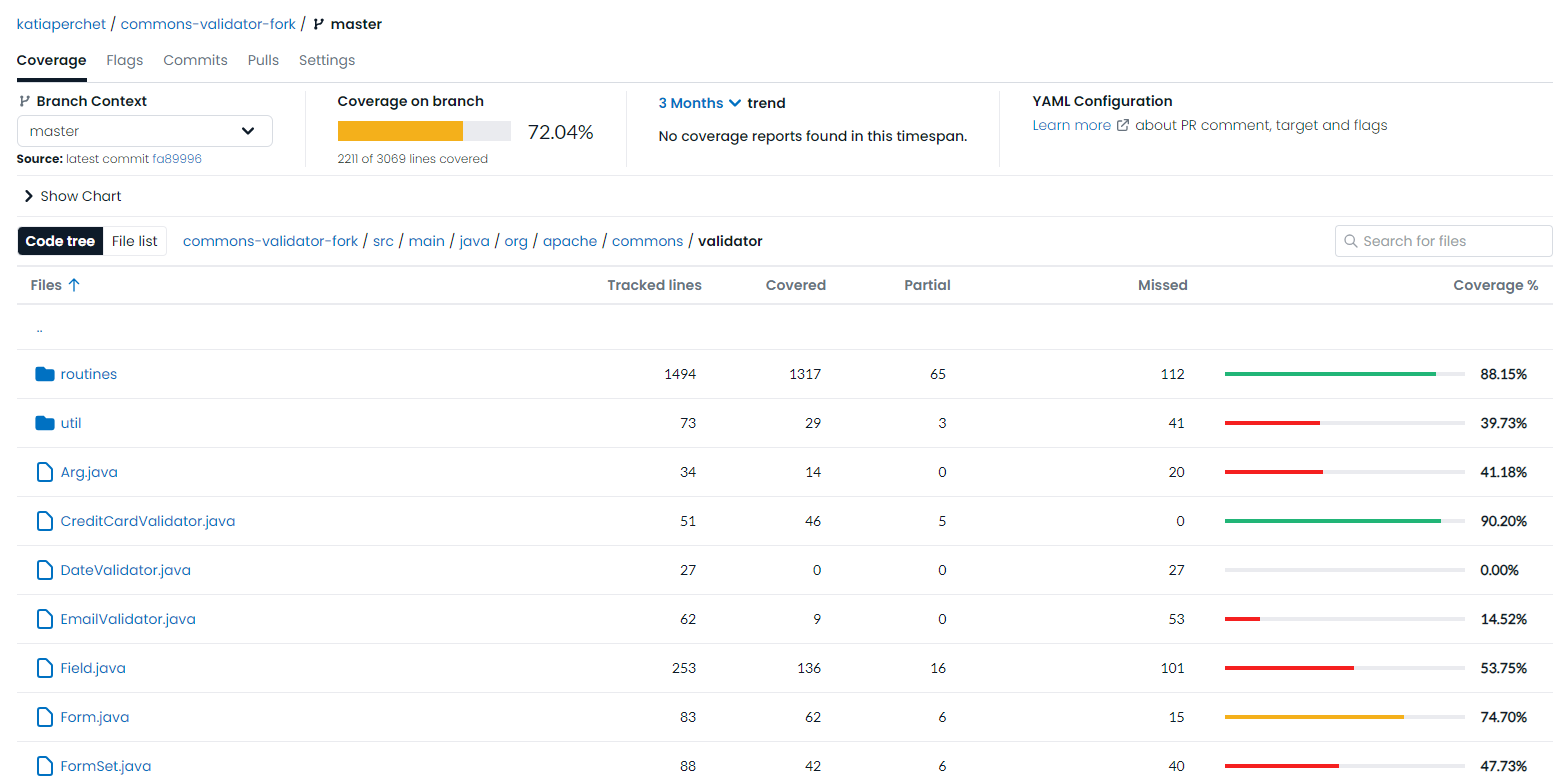
\includegraphics[width=1\columnwidth]{codecov.png}
    \caption{CodeCov generated report.}
    \label{fig:enter-label}
\end{figure}

\section{4. Mutation Testing}
Mutation testing serves as a critical measure to evaluate the effectiveness of a test suite by introducing artificial faults or mutations into the source code. In this pursuit, PiTest has been implemented to systematically alter the production code, inducing intentional faults and gauging the test suite's ability to detect and report these mutations through test failures.

\subsection{4.1 PiTest}
PiTest \cite{pitest} stands as an open-source mutation testing tool designed for Java applications. Employing advanced testing techniques, it aims to enhance test adequacy and pinpoint defects within the codebase. By revealing weaknesses in test coverage, PiTest empowers developers to enhance both the overall code quality and reliability. 

\subsection{4.2 PiTest Report}
The generated report presents these findings as the project summary, incorporating an analysis of 61 total classes.

\begin{figure}[h!]
    \centering
    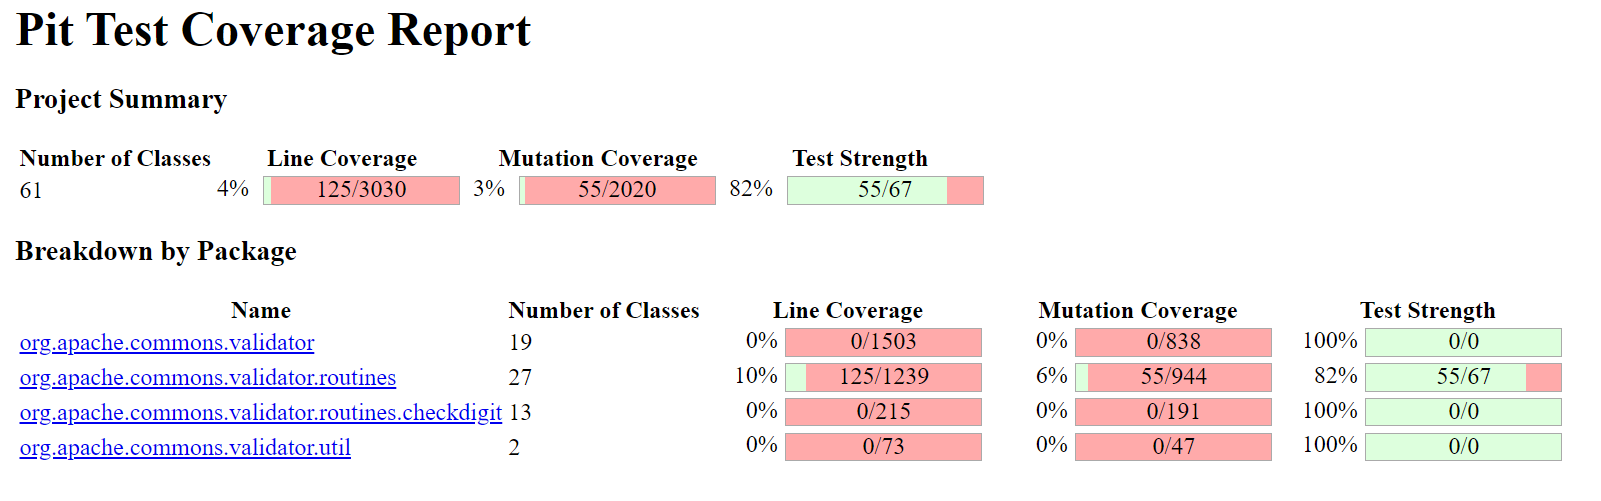
\includegraphics[width=1\columnwidth]{pitest1.png}
    \caption{PiTest generated report.}
    \label{fig:enter-label}
\end{figure}

\subsubsection{\textbf{Mutant Coverage}}
The mutant coverage denotes the percentage of potential bugs identified by the production code, and in the case of Apache Commons Validator, it is notably low. The comprehensive mutation coverage for the entire project revealed that only 3\% of the introduced mutants (55 out of 2020) were successfully detected. The majority of detections occurred within the "routines" package, particularly in the "DomainValidator.java" class, where 43 out of 84 mutants were successfully identified, and the "RegexValidator.java" class, where 12 out of 35 mutants were detected successfully.

\subsubsection{\textbf{Line Coverage}}
The line coverage for the entire project is notably low, with only 4\% of the codebase's statements covered by the test cases, amounting to 125 out of 3030 lines. The majority of this coverage is within the "routines" package, particularly in the "DomainValidator.java" class, where 104 out of 179 lines were covered, and the "RegexValidator.java" class, where 21 out of 59 lines were successfully covered.

\subsubsection{\textbf{Test Strength}}
The overall test strength of the project, indicating the percentage of mutations eliminated by tests relative to the total mutations covered by tests, is high. Out of 67 mutations covered by tests, 55 were successfully eliminated, representing an 82\% test strength. The majority of these eliminations occurred in the "routines" package, particularly in the "DomainValidator.java" class, where 43 out of 54 mutations were detected and killed, and the "RegexValidator.java" class, where 12 out of 13 mutations were successfully detected and eliminated.

\section{5. Benchmarking Tools}
Benchmarking tools helps to identify areas for improvement, make informed decisions, and ensure that systems meet certain standards or requirements. In this context, Java Microbenchmark Harness (JMH) was implemented to provide a quantitative and objective basis for assessing the capabilities and limitations of the project.

\subsection{5.1 Java Microbenchmark Harness}
Java Microbenchmarking Harness (JMH)\cite{jmh} stands out as a robust and versatile tool designed for the precise and dependable benchmarking of Java code, with a specific emphasis on microbenchmarks, facilitating accurate measurement and analysis within a controlled and well-defined framework. 

Its objective lies in orchestrating benchmarking activities within controlled environments, presenting developers with valuable and trustworthy insights into the performance nuances of their codebase.

After a comprehensive analysis within the context of the input validator project, it becomes apparent that the tests validating URLs for correctness in terms of format and authority consume the most system resources. Subsequently, scenarios involving varying URI lengths and validations distinctly demonstrate lower performance.

Two benchmark methods were introduced to measure the performance of two variations of authorization and URL validation using JMH. In all the methods, the benchmark mode employed was "Throughput" which facilitated the measurement of how many operations were performed in a unit of time, in this case, operations per second. It is noteworthy that each method underwent 25 benchmark iterations.

It is evident that the introduced URI can significantly impact the performance results. When a non-existent URI is used, the analysis and performance measurements are considerably lower compared to using the URI of an existing web page. For instance, methods like "testIsValid1Benchmark" and "testIsValidAuth1Benchmark" exhibit higher scores than "testIsValid2Benchmark" and "testIsValidAuth2Benchmark." The key distinction is that tests in group 1 involved sending the URI of Google, while tests in group 2 used a hypothetical URI.

\begin{figure}[h!]
    \centering
    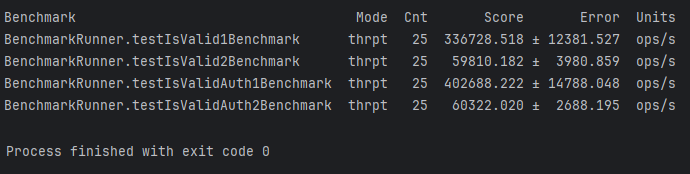
\includegraphics[width=1\columnwidth]{benchmark1.png}
    \caption{JMH generated report.}
    \label{fig:enter-label}
\end{figure}

\section{6. Automated Testing Generation Tools}
Automated test case generation is key to boosting the quality, reliability, and maintainability of a Java project. It efficiently explores, validates, and documents the system's behavior, contributing to a strong and effective software development process.  In this context, EvoSuite was utilized to automatically generate fundamental unit tests with assertions for classes. Employing evolutionary algorithms, such as genetic algorithms, it evaluates numerous plausible test suites for a given class and provides what it deems as the best one.


\subsection{6.1 EvoSuite}
EvoSuite \cite{evosuite} aims to generate test suites with two primary goals: maximizing a specified coverage criterion, like branch coverage, and minimizing the suite's size in terms of the number of tests and statements. Once it provides a test suite, EvoSuite can additionally propose sets of assertions for each test case using mutation analysis. These assertions serve to encapsulate the existing behavior of the tested code, making them valuable for regression testing.

Utilizing EvoSuite, the Apache Commons Validator project benefited from the efficient generation of automated tests. This process resulted in the creation of 129 new tests for enhanced code coverage. Each class was equipped with two types of tests: the primary test and accompanying scaffolding classes. These scaffolding classes serve to provide essential infrastructure and methods supporting the generated tests. Notably, they contribute to the independence and isolation of the generated tests from those created manually.


\section{7. Software Vulnerabilities}

A software vulnerability represents a potential security risk within a software system, and understanding, identifying, and addressing these vulnerabilities is essential for ensuring the security and reliability of software applications. 
There are common types of vulnerabilities found in software project, including in Apache Commons Validator.
\begin{itemize}
    \item \textbf{Injection Vulnerabilities:} occur when user inputs are not rigorously validated and sanitized. In such scenarios, attackers can exploit these weaknesses to inject malicious code into the application. Robust input validation and sanitization processes are crucial to mitigate the risks associated with injection vulnerabilities.
    \item \textbf{Denial of Service (DoS):} attacks aim to disrupt the normal functioning of a system by overwhelming it with a barrage of requests or by exploiting specific weaknesses. This can lead to a temporary or prolonged unavailability of services, impacting the user experience and potentially causing financial losses.
    \item \textbf{Buffer Overflows:} represent a classic vulnerability that occurs when a program writes more data to a block of memory, known as a buffer, than it was allocated for. This can lead to potential code execution, allowing attackers to manipulate the program's behavior and compromise the security of the system. 
\end{itemize}

\subsection{7.1 Find Security Bugs}
Find Security Bugs \cite{findsecbugs} operates as an automated security analysis tool, leveraging its capabilities to scrutinize Java code comprehensively. Incorporating Find Security Bugs into the development contributes to the creation of resilient and secure Java applications.

\subsubsection{\textbf{7.1.1 FindSecBugs Report}}
When integrated into the Apache Commons Validator project, the report uncovered a several issues tied to regular expressions (regex) and their excessive length. This extended length raised concerns about potential Denial of Service (DoS) vulnerabilities, especially when dealing with large user inputs. The problem arises from the fact that the Regex engine can consume a considerable amount of processing time when analyzing specific string configurations, creating a window for potential DoS attacks. SonarCloud also flagged this vulnerability during its initial analysis.

To mitigate this, the best option is to rewrite the regex expressions. By streamlining and optimizing them, we can enhance the accuracy of input validation and sidestep the risks associated with prolonged regex processing times. This proactive approach of revamping regex patterns is key to make more robust the Apache Commons Validator project and ensuring it handles a variety of user inputs securely.

\begin{figure}[h!]
    \centering
    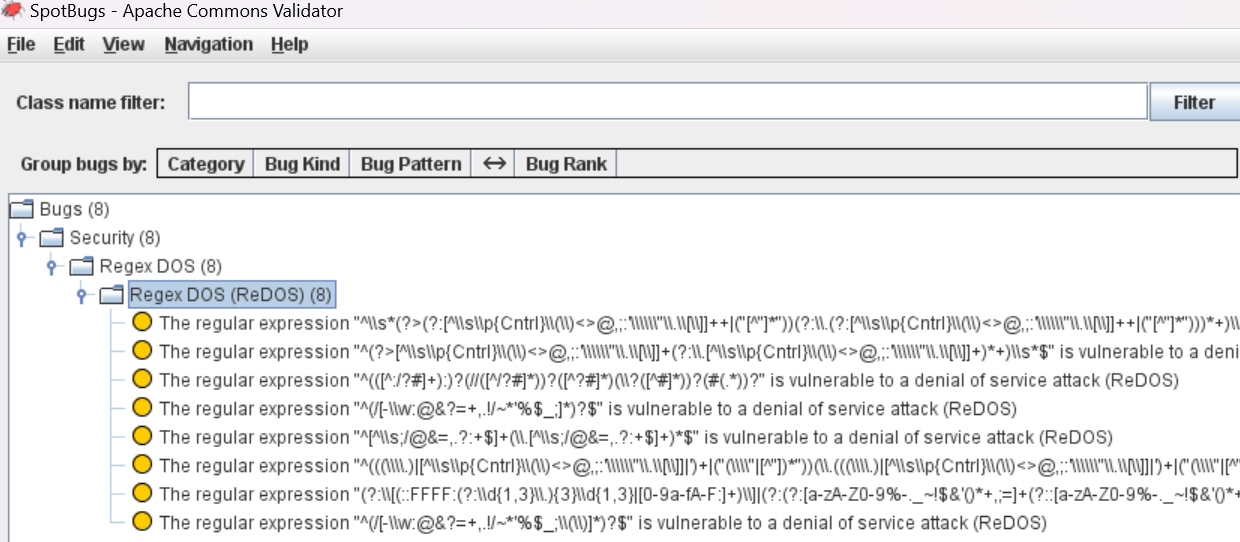
\includegraphics[width=1\columnwidth]{findsecbugs.png}
    \caption{FindSecBugs generated report.}
    \label{fig:enter-label}
\end{figure}

\subsection{7.2 OWASP Dependency Check}
When implemented OWASP Dependency-Check \cite{owasp-dependency-check} it helped to identify and mitigate security risks associated with third-party dependencies. It promotes secure coding practices and helped to make informed decisions regarding the use of third-party components on the Apache Commons Validator project.
\subsubsection{\textbf{7.2.1 Dependency Overview}}
After conducting a comprehensive analysis using OWASP Dependency Checker (version 9.0.4), the generated report identified nine unique dependencies, each essential for the project's functionality. Fortunately, the thorough examination revealed that none of these dependencies harbored vulnerabilities, ensuring the overall security integrity of the project.

\begin{figure}[h!]
    \centering
    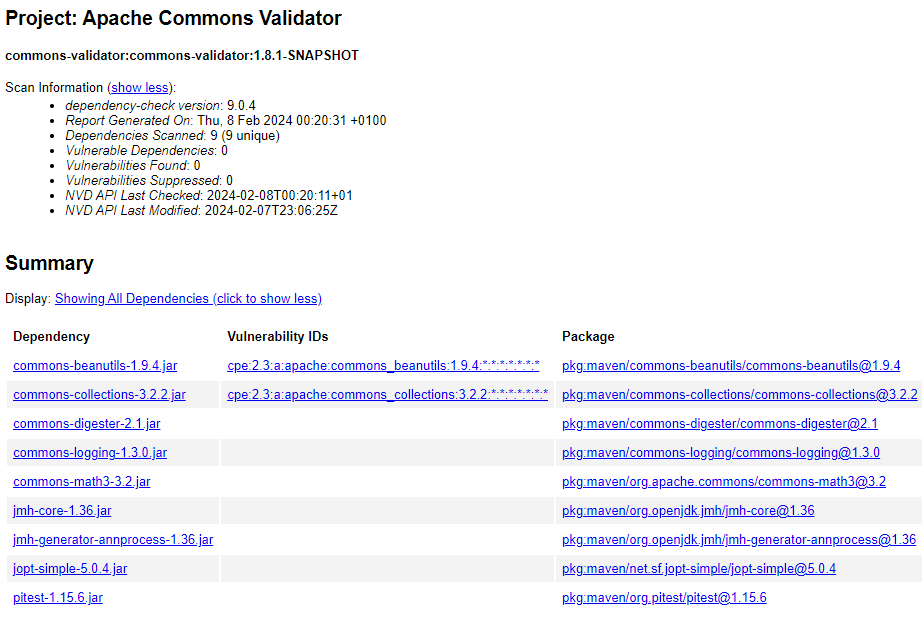
\includegraphics[width=1\columnwidth]{owaspReport2.png}
    \caption{OWASP Dependency Check - HTML generated report.}
    \label{fig:enter-label}
\end{figure}

\subsubsection{\textbf{7.2.2 Summary of Dependencies}}
\begin{itemize}
    \item \textbf{Apache Commons BeanUtil 1.9.4.} Library for streamlined manipulation and handling of JavaBeans components. It simplifies Java object-related operations and promotes code reusability.
    \begin{itemize}
        \item Analysis: The analysis highlighted it as one of the dependencies with the highest confidence. With an evidence count of 168.
    \end{itemize}
    
    \item \textbf{Apache Commons Collections 3.2.2.} Library that provides additional collection types and utilities for working with Java collections. It offers various data structures, algorithms, and decorators to enhance the functionality of standard Java collections.
    \begin{itemize}
        \item Analysis: The analysis highlighted it as one of the dependencies with the highest confidence. With an evidence count of 84.
    \end{itemize}
    \item \textbf{Apache Commons Digester 2.1.} Library designed for processing XML documents using a rule-based approach. It simplifies XML parsing and provides a flexible mechanism for mapping XML elements to Java objects based on configurable rules.
    \begin{itemize}
        \item Analysis: The analysis highlighted it as a dependency with the high confidence. With an evidence count of 98.
    \end{itemize}
    \item \textbf{Apache Commons Logging 1.3.0.} It provides a common interface for logging operations. By offering a thin abstraction layer, it enables greater flexibility in choosing and switching between different logging frameworks without modifying application code.
    \begin{itemize}
        \item Analysis: The analysis highlighted it as a dependency with the high confidence. With an evidence count of 129.
    \end{itemize}
    \item \textbf{Apache Commons Math 3-3.2.} Library that provides mathematical functionalities for Java applications. It includes a wide range of mathematical operations, algorithms, and utilities, covering areas such as linear algebra, statistics, optimization, and numerical analysis. 
    \begin{itemize}
        \item Analysis: The analysis highlighted it as a dependency with the high confidence. With an evidence count of 125.
    \end{itemize}
    \item \textbf{JMH (Java Microbenchmarking Harness) Core 1.36.}  Component of the OpenJDK project that provides a robust framework for benchmarking Java code. It is widely used for measuring and analyzing the runtime behavior of code snippets, methods, or entire programs, helping to optimize and fine-tune Java applications for better performance.
    \begin{itemize}
        \item Analysis: The analysis highlighted it as a dependency with the high confidence. With an evidence count of 27.
    \end{itemize}
    \item \textbf{JMH Generator Annprocess 1.36.} Component of JMH that serves as an annotation processor. It is designed to process annotations related to JMH benchmarks during the compilation phase of a Java project.
    \begin{itemize}
        \item Analysis: The analysis highlighted it as a dependency with the high confidence. With an evidence count of 25.
    \end{itemize}
    \item \textbf{Jopt Simple 5.0.4.} Java library that provides a simple and lightweight framework for parsing command-line options and arguments. The library allows for the definition of command-line options, parsing user input, and handling various types of command-line arguments. With its straightforward approach, jopt-simple simplifies the process of creating command-line interfaces.
    \begin{itemize}
        \item Analysis: The analysis highlighted it as a dependency with the high confidence. With an evidence count of 23.
    \end{itemize}
    \item \textbf{PiTest 1.15.6}  It introduces artificial faults or mutations into the source code to evaluate the effectiveness of test suites. By dynamically modifying the production code, PiTest helps identify weaknesses in test coverage, allowing developers to enhance the overall quality and reliability of their Java applications.
    \begin{itemize}
        \item Analysis: The analysis highlighted it as a dependency with the high confidence. With an evidence count of 23.
    \end{itemize}
\end{itemize}
\subsubsection{\textbf{7.2.3. Summary of OWASP DC}}
In conclusion, the implementation of OWASP Dependency Check for the project's dependencies provided valuable insights, revealing the importance of proactive dependency management and the effectiveness of tools like OWASP Dependency Check in maintaining a secure and robust software ecosystem. The Apache Commons Validator can confidently rely on these dependencies to deliver its features without compromising security.

\section{8. Conclusion}

To sum up, the comprehensive application of SonarCloud, JaCoCo, PiTest, JMH, EvoSuite, FindSecBugs, and OWASP Dependency Check to the Apache Commons Validator project has significantly enhanced its overall quality, reliability, and security. 

SonarCloud played a pivotal role in identifying and rectifying code quality issues, while JaCoCo provided insightful code coverage metrics, ensuring thorough testing. PiTest, through mutation testing, pinpointed potential weaknesses in the test coverage, enabling to fortify the code against defects.

JMH facilitated precise and reliable benchmarking, allowing for performance optimization. EvoSuite's automated test generation contributed to the creation of a robust test suite, improving code coverage and identifying potential vulnerabilities. FindSecBugs efficiently detected security bugs, fortifying the project against potential threats. Finally, OWASP Dependency Check ensured that the project's dependencies were free from vulnerabilities, contributing to a secure and resilient software ecosystem. 

The combined implementation of these tools has significantly elevated the project's dependability, providing a solid foundation for its continued development and deployment. It is imperative to acknowledge that these practices and implementations should be continuously employed as an integral part of the development life cycle. This ongoing commitment to utilizing these tools ensures sustained dependability, optimal performance, and the continued implementation of best practices. Adopting these practices as part of a continuous improvement strategy will not only fortify the existing project but also set the stage for future development endeavors, promoting a culture of excellence and resilience in software engineering.

\section{Acknowledgments}
To everyone who provided guidance for this project.




% BALANCE COLUMNS
\balance{}

% REFERENCES FORMAT
% References must be the same font size as other body text.
\bibliographystyle{SIGCHI-Reference-Format}
\bibliography{sample}

\end{document}

%%% Local Variables:
%%% mode: latex
%%% TeX-master: t
%%% End:
